量子计算是一个快速发展的领域，有望深刻改变我们处理信息的方式。不同于使用比特表示信息的经典计算机，量子计算机使用量子比特。由于量子叠加，量子比特能够同时编码多个计算基态，使量子计算机在某些计算任务上远快于经典计算机。此类算法包括 Grover 搜索算法 \cite{grover1996fast, long2001grover}、Shor 因数分解算法 \cite{shor1994algorithms} 和 HHL 线性方程组求解算法 \cite{harrow2009quantum}。近年来，量子计算芯片发展相对迅速。IBM 先后推出了 433 量子比特 Osprey 量子芯片 \cite{ibm2022osprey} 和 1121 量子比特 Condor 量子芯片 \cite{castelvecchi2023ibm}。Google 也在 53 量子比特 Sycamore 量子芯片上展示了量子优越性 \cite{arute2019quantum}。中国也发布了 66 量子比特可编程量子计算芯片 Zuchongzhi-2 \cite{wu2021strong}。如何高效使用这些量子芯片，已经成为日益重要的研究课题。

目前，我们仍处于 NISQ 量子计算阶段 \cite{preskill2018quantum}。量子计算机中的量子比特数量仍然相对有限，量子门也存在噪声。因此，利用 CPU、GPU 和昇腾（Ascend）等经典硬件进行量子模拟十分重要。借助量子模拟器，我们可以快速开发并验证量子算法。此外，我们还可以使用量子模拟器验证量子芯片的正确性，或辅助完成当前含噪量子芯片上的误差缓解。

在 NISQ 阶段，一类称为量子-经典混合变分算法的变分量子算法 \cite{Peruzzo2014Peruzzo2014,cerezo2021variational,PhysRevA.109.052414} 可能具有更高的实际应用价值。这类算法对噪声具备一定鲁棒性，包括用于模拟化学分子的变分量子本征求解器 \cite{mcardle2020quantum,cao2019quantum,yeter2020practical,fan2023circuit}、用于求解组合优化问题的量子近似优化算法 \cite{farhi2014quantum,PhysRevResearch.4.013141}，以及用于处理分类与模式生成任务的量子机器学习算法 \cite{benedetti2019parameterized,biamonte2017quantum,das2019machine,PhysRevResearch.6.013027}。根据变分算法的原理，变分量子算法依赖经典优化器调节变分量子线路中的参数，使量子系统输出尽可能接近期望目标，从而达到优化学习的目的。

本文提出一个名为 MindSpore Quantum（\MindQuantum）的量子-经典混合编程框架。相较于 QuEST \cite{jones2019quest}、QPanda \cite{dou2022qpanda}、TensorCircuit \cite{zhang2023tensorcircuit}、Qulacs \cite{suzuki2021qulacs}、TensorFlow Quantum \cite{broughton2020tensorflow}、Yao \cite{luo2020yao}、Intel Quantum Simulator \cite{guerreschi2020intel} 和 PennyLane \cite{bergholm2018pennylane} 等其他量子框架，\MindQuantum\ 提供了简洁、易用且高效的量子编程框架，支持量子线路的构造、模拟以及基于真实芯片的执行。结合 MindSpore，用户可以快速开发并训练量子-经典混合算法。图~\ref{fig:framework} 展示了 \MindQuantum\ 的总体架构。

\definecolor{c8adacd}{RGB}{138,218,205}
\definecolor{ce8f8f3}{RGB}{232,248,243}
\definecolor{cffc46d}{RGB}{255,196,109}
\definecolor{cf2f2f2}{RGB}{220,220,220}
\definecolor{c6de1ff}{RGB}{109,225,255}
\definecolor{caffaeb}{RGB}{175,250,235}
\definecolor{c0157b4}{RGB}{1,87,180}
\def \globalscale {1.000000}
\begin{figure*}
    \begin{tikzpicture}[scale=0.6, every node/.append style={scale=\globalscale}, inner sep=0pt, outer sep=0pt]
        % Basic Component
        \path[draw=black,line width=0.0794cm] (0.0397, 29.1174) rectangle (29.2232, 17.8991);
        \node[align=center, font=\bfseries] at (14.63145, 28.5174) {基本组件};

        \path[fill=c8adacd, draw] (0.4895, 28.0061) rectangle (7.3686, 27.0272);
        \node[align=center] at (3.92905, 27.51665) {量子门};


        \path[fill=ce8f8f3] (0.4763, 26.8023) rectangle (7.3819, 18.2563);
        \node[draw=none] at (4.2, 25) {
            \begin{minipage}{0.3\textwidth}
                \begin{itemize}
                    \item 固定门
                    \item 参数化门
                    \item 任意门控制
                    \item 噪声信道
                \end{itemize}
            \end{minipage}
        };
        \path[fill=white,rounded corners=0.6879cm] (0.926, 22.8865) rectangle (6.9321, 18.6796);


        \path[fill=c8adacd, draw] (7.6332, 28.0061) rectangle (14.4859, 27.0272);
        \node[align=center] at (11.05955, 27.51665) {量子线路};

        \path[fill=ce8f8f3] (7.62, 26.8023) rectangle (14.5256, 18.2563);
        \node[draw=none] at (11.3437, 25.5) {
            \begin{minipage}{0.3\textwidth}
                \begin{itemize}
                    \item append 操作
                    \item $+=$ 运算符
                    \item 链式规则
                \end{itemize}
            \end{minipage}
        };
        \path[fill=white,rounded corners=0.6879cm] (8.0698, 22.8865) rectangle (14.0758, 18.6796);

        \path[fill=c8adacd, draw] (14.777, 28.0061) rectangle (21.6561, 27.0272);
        \node[align=center] at (18.21655, 27.51665) {参数解析器};
        \path[fill=ce8f8f3] (14.7638, 26.8023) rectangle (21.6694, 18.2563);
        \node[draw=none] at (18.4875, 25.9) {
            \begin{minipage}{0.3\textwidth}
                \begin{itemize}
                    \item 微调
                    \item 算术运算
                \end{itemize}
            \end{minipage}
        };
        \path[fill=white,rounded corners=0.6879cm] (15.2135, 22.8865) rectangle (21.2196, 18.6796);

        \path[fill=c8adacd, draw] (21.9207, 28.0061) rectangle (28.7734, 27.0272);
        \node[align=center] at (25.34705, 27.51665) {可观测量};
        \path[fill=ce8f8f3] (21.9075, 26.8023) rectangle (28.8131, 18.2563);
        \node[draw=none] at (25.6312, 25) {
            \begin{minipage}{0.3\textwidth}
                \begin{itemize}
                    \item 哈密顿量
                    \item QubitOperator
                    \item FermionOperator
                    \item 变换
                \end{itemize}
            \end{minipage}
        };
        \path[fill=white,rounded corners=0.6879cm] (22.3573, 22.8865) rectangle (28.3633, 18.6796);
        \node at (3.92905, 20.78305) {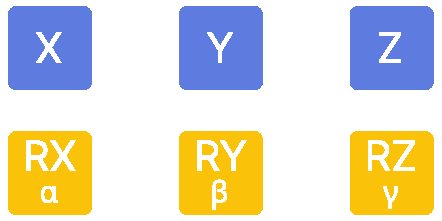
\includegraphics[scale=0.4]{images/1_1_1.pdf}};
        \node at (11.07285, 20.78305) {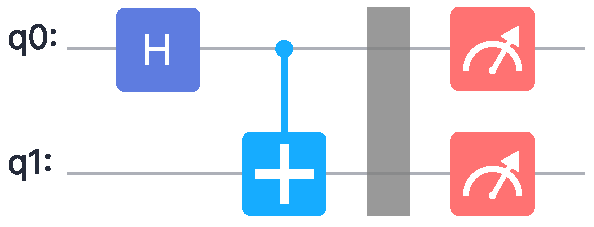
\includegraphics[scale=0.35]{images/1_1_2.pdf}};
        \node at (18.21665, 21.18305){
            \begin{minipage}{0.22\textwidth}
                \ttfamily\scriptsize
                a, b = np.pi, 0.5\\
                ParameterResolver(\{\\
                \hspace*{1em}'a': a, 'b': b\\
                \})
            \end{minipage}
        };

        \node[align=center] at (18.21665, 19.68305) {\textcolor{blue}{$\pi * a+ 1 / 2 * b$}};
        \node at (25.36045, 21.18305-0.2){
            \begin{minipage}{0.22\textwidth}
                \ttfamily\scriptsize
                o = QubitOperator(\\
                \hspace*{1em}'X0 Y1', 'a'\\
                ) + QubitOperator(\\
                \hspace*{1em}'Z2', np.sqrt(2)\\
                )
            \end{minipage}
        };
        \node[align=center] at (25.36045, 19.68305-0.2) {\textcolor{blue}{$aX_0Y_1 + \sqrt{2}Z_2$}};

        % NISQ
        \path[draw=black,line width=0.0794cm] (0.0397, 17.608) rectangle (14.4595, 10.2791);
        \node[align=center, font=\bfseries] at (7.2496, 17.008) {NISQ 算法};

        \path[fill=cffc46d,draw] (0.5159, 16.047) rectangle (6.9453, 14.7505);
        \node[align=center] at (3.7306, 15.39875) {Ansatz 库};

        \path[draw=black] (0.5159, 14.7241) rectangle (6.9453, 10.5436);

        \path[fill=cffc46d,draw] (7.62, 16.0602) rectangle (14.0758, 14.7373);
        \node[align=center] at (10.8479, 15.39875) {VQE};

        \path[fill=cffc46d, draw] (7.62, 13.9435) rectangle (14.0758, 12.6206);
        \node[align=center] at (10.8479, 13.28205) {QAOA};

        \path[fill=cffc46d, draw] (7.62, 11.8269) rectangle (14.0758, 10.504);
        \node[align=center] at (10.8479, 11.16545) {QNN};
        \node at (3.7306, 12.58205) {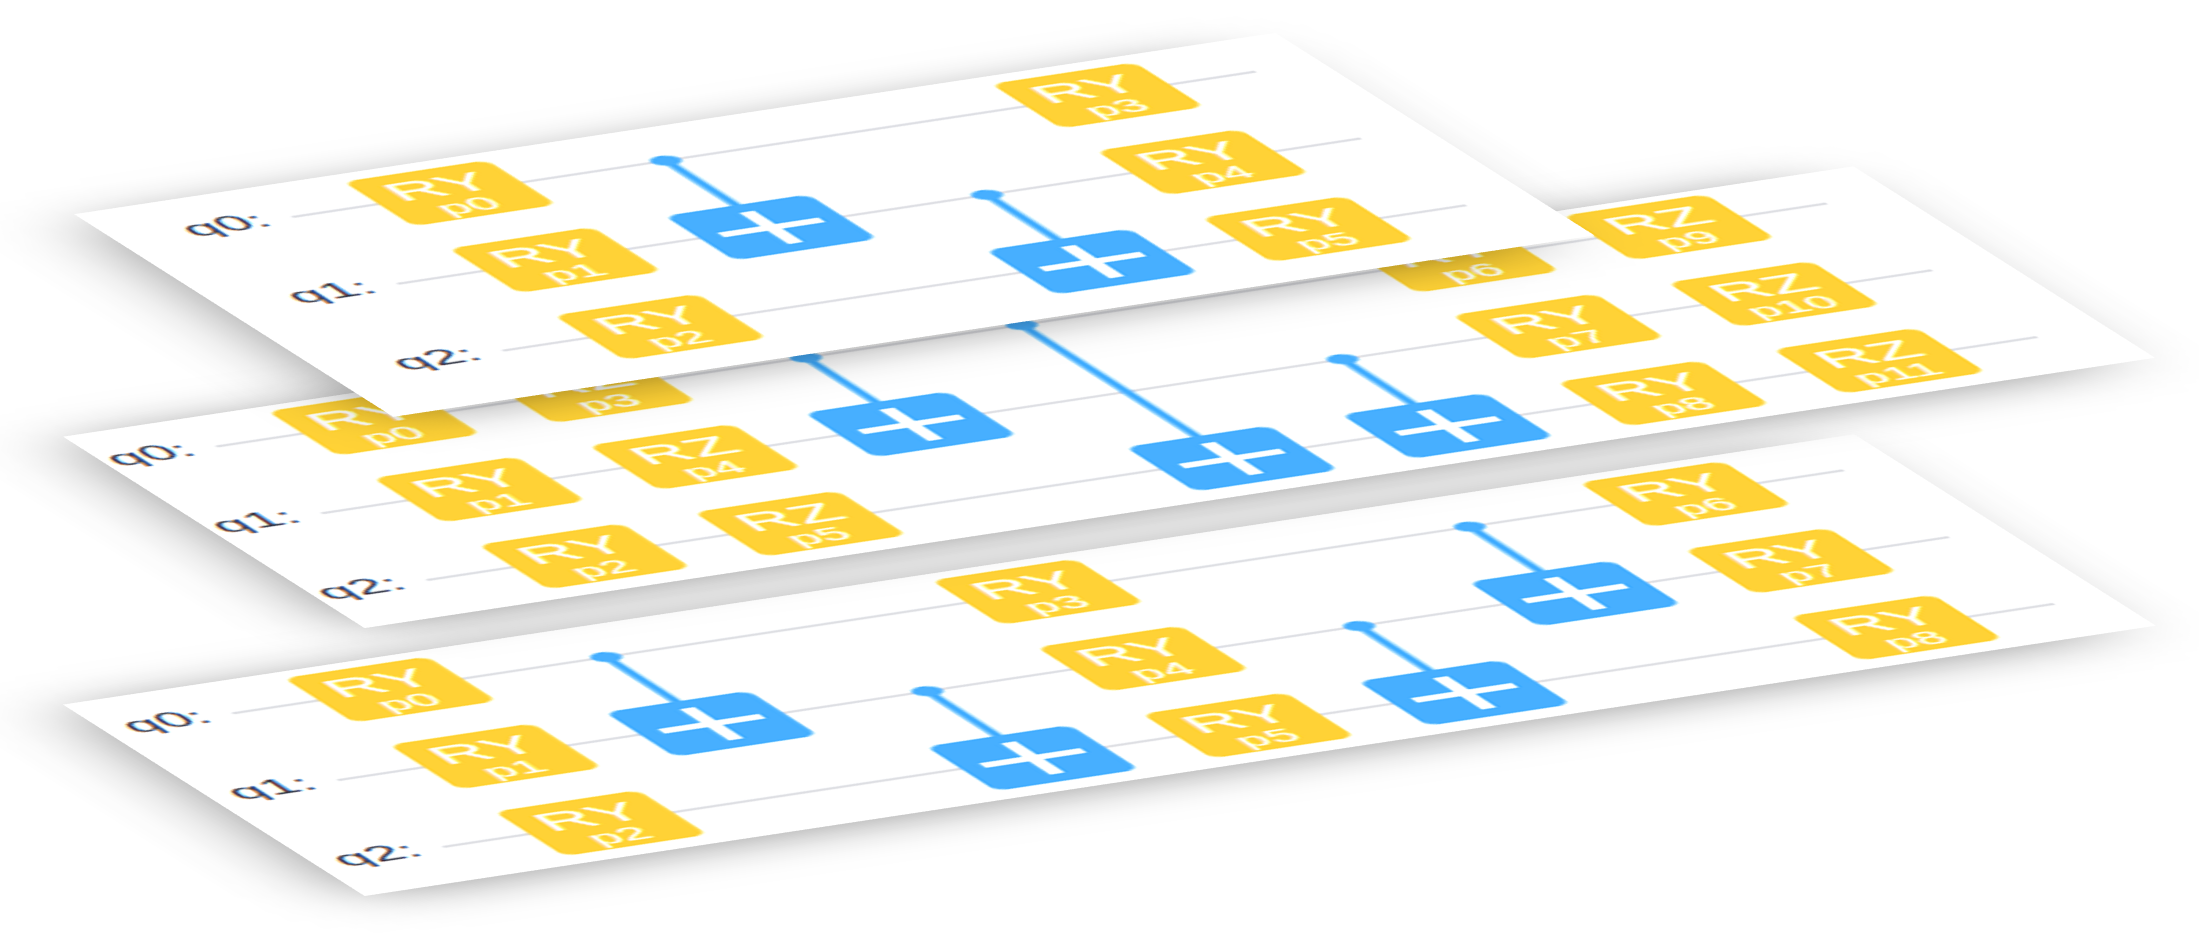
\includegraphics[scale=0.065]{images/1_1_4.jpeg}};


        % Compiler
        \path[draw=black,line width=0.0794cm] (14.8034, 17.608) rectangle (29.2232, 10.2791);
        \node[align=center, font=\bfseries] at (22.0133, 17.008) {编译算法};

        \path[fill=cffc46d,draw] (19.7379, 15.2929) rectangle (28.3633, 13.97);
        \node[align=center] at (24.0506, 14.63145) {基于 DAG 的线路编译器};

        \path[fill=cffc46d,draw] (19.7379, 12.4883) rectangle (28.3633, 11.1654);
        \node[align=center] at (24.0506, 11.82685) {量子比特映射};
        \node at (17.2506, 13.22915) {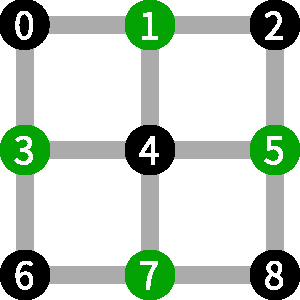
\includegraphics[scale=0.5]{images/1_1_3.pdf}};

        % simulator
        \path[draw=black,line width=0.0794cm] (0.0397, 9.8822) rectangle (14.4595, 3.2941);
        \node[align=center, font=\bfseries] at (7.2496, 9.2822) {量子模拟器};

        \path[fill=c6de1ff] (0.4895, 8.5328) rectangle (14.0626, 7.2364);
        \node[align=center] at (7.2496, 7.8846) {核心模拟算法};

        \path[fill=caffaeb] (0.4763, 6.9585) rectangle (14.0758, 3.5719);
        \node[draw=none] at (5.7, 5.2415) {
            \begin{minipage}{0.4\textwidth}
                \begin{itemize}
                    \item 线路演化
                    \item 采样测量
                    \item 可观测量期望值
                    \item 批模式梯度计算
                \end{itemize}
            \end{minipage}
        };

        % cpu_gpu
        \path[draw=black,line width=0.0794cm] (0.0661, 2.8972) rectangle (14.4859, 0.0397);
        \node[align=center, font=\bfseries] at (7.276,2.2972) {策略细节};

        \path[fill=c0157b4] (0.2646, 1.7992) rectangle (4.6038, 0.2117);
        \node[align=center,text=white] at (2.4342,1.00545) {X86(AVX)};

        \path[fill=c0157b4] (5.0271, 1.7992) rectangle (9.3663, 0.2117);
        \node[align=center,text=white] at (7.1967,1.00545) {GPU(CUDA)};

        \path[fill=c0157b4] (9.7896, 1.7992) rectangle (14.1288, 0.2117);
        \node[align=center,text=white] at (11.9592,1.00545) {Ascend(NENO)};


        % provider
        \path[fill=cf2f2f2] (14.8034, 9.8822) rectangle (29.2232, 3.2941);
        \path[draw=black,line width=0.0794cm,dash pattern=on 0.1588cm off 0.1588cm] (14.8034, 9.8822) rectangle (29.2232, 3.2941);
        \node[align=center, font=\bfseries] at (22.0133, 6.58815) {后端提供者};

        % QPU
        \path[fill=cf2f2f2] (14.8034, 2.8972) rectangle (29.2232, 0.0397);
        \path[draw=black,line width=0.0794cm,dash pattern=on 0.1588cm off 0.1588cm] (14.8034, 2.8972) rectangle (29.2232, 0.0397);
        \node[align=center, font=\bfseries] at (22.0133, 1.46845) {QPU};

    \end{tikzpicture}
    \caption{\MindQuantum\ 的框架}
    \label{fig:framework}
\end{figure*}


\begin{description}
    \item[第一层] 这一层表示框架的基础构件。我们提供多种量子门，以及构造量子线路的便捷方式。为支持变分量子算法，我们还提供参数解析器，用于将部分量子门转换为变分量子门。此外，我们还提供描述各类可观测量的能力。
    \item[第二层] 这一层是算法层，包含通用量子算法和变分量子算法。此外，该层还包括量子编译算法，用于将量子线路编译并映射到量子芯片。
    \item[第三层] 这一层是执行层，会根据执行所使用的硬件划分为量子模拟器和量子芯片后端提供者。在量子模拟器中，我们针对 CPU、GPU 和昇腾架构设计了高性能模拟逻辑，并支持在单精度和双精度模拟模式之间灵活切换。
\end{description}

本白皮书的结构安排如下：第 \hyperref[sec:elements]{\ref*{sec:elements}} 章将介绍 \MindQuantum\ 中用于构造量子线路和可观测量的基本元素；第 \hyperref[sec:backend]{\ref*{sec:backend}} 章将全面展示量子模拟器的使用方法，包括通用状态矢量模拟、密度矩阵模拟、量子化学 CI 子空间模拟和含噪模拟；第 \hyperref[sec:toolbox]{\ref*{sec:toolbox}} 章将讨论 \MindQuantum\ 中与变分量子算法相关的模块，包括各种类型的变分量子线路，以及求解变分量子线路梯度的方法；第 \hyperref[sec:applications]{\ref*{sec:applications}} 章将展示当前学术界近期研究成果中使用 \MindQuantum\ 的示例；第 \hyperref[sec:benchmark]{\ref*{sec:benchmark}} 章将在不同场景中对 \MindQuantum\ 与若干其他量子计算框架进行性能基准比较；第 \hyperref[sec:chip]{\ref*{sec:chip}} 章将说明如何利用 \MindQuantum\ 在真实量子芯片上运行量子算法；第 \hyperref[sec:summary]{\ref*{sec:summary}} 章将对全文进行总结。最后，在第 \hyperref[sec:acknowledgement]{\ref*{sec:acknowledgement}} 章中，我们将感谢所有为 \MindQuantum\ 作出贡献的人，以及在研究中使用 \MindQuantum\ 的用户。
